\documentclass[a4paper,10pt,twoside]{book}
\usepackage[utf8]{inputenc}
\usepackage[english]{babel}
\usepackage{graphicx}
\usepackage[table]{xcolor}
\usepackage{geometry}
\usepackage{multirow}
\usepackage{booktabs}
\usepackage{float}
\usepackage{csquotes}
\usepackage{hyperref}
\usepackage{listings}
\usepackage[backend=biber]{biblatex}
\addbibresource{refs.bib}
\graphicspath{ {./images/} }
\geometry{
	left=20mm,
	right=15mm,
	top=20mm,
	bottom=15mm,
	heightrounded,
	}
\setlength{\parindent}{0.5cm}
\setcounter{secnumdepth}{3}
\newcommand\tab[1][1cm]{\hspace*{#1}}
\newcommand*{\thead}[1]{\multicolumn{1}{|c|}{\bfseries #1}}
\newcommand{\tabitem}{~~\llap{\textbullet}~~}
\begin{document}

\author{Avijit Naskar}
\title{CS101: All in one book for Competitive Exam}
\date{January 2025}

\frontmatter
\maketitle
\tableofcontents
\mainmatter
\part{Discrete Mathematics}

\chapter{Mathematical Logic}

\chapter{Linear Algebra}

\chapter{Graph Theory}
\section{Graphs}
\subsection{Terminologies}
\begin{itemize}
	\item \textbf{Graph} A graph G=(V,E) consists of a set of objects $V={v_1,v_2,v_3,...}$ called vertices and $E={e_1,e_2,e_3,...}$ called edges.
	\item \textbf{Edges} An edge $e_k$ is an unordered pair of vertices $(v_i,v_j)$.
	\item \textbf{Vertex} Vertices are the nodes/points of both sides of edges.
	\item \textbf{Adjacent Vertices} If two vertices connected with same edge.
	\item \textbf{Degree or Valency} Number of edges incident on a vertex
	\item \textbf{Regular Graph} A graph which has all vertices of same degree
	\item \textbf{Isolated Vertex} A vertex of degree zero
	\item \textbf{Pedant Vertex} A vertex of degree one
	\item \textbf{Common Vertex} A vertex 
	\item \textbf{Null Graph} A graph with no edges
\end{itemize}
\subsection{Theorems}
\begin{enumerate}
	\item The sum of degrees of all vertices in a graph: $\sum_{i=1}^{n}d(v_i)=2e$
	\item The number of vertices of odd degree in a graph is always even
\end{enumerate}
\subsection{Planner graphs} 

\chapter{Set Theory}

\chapter{Group Theory}

\chapter{Optimization}

\chapter{Probability}
\section{Probability Basics}
\section{Distributions}
\subsection{Uniform Distribution}
\subsection{Random Distribution}
\subsection{Exponential Distribution}
\subsection{Poisson Distribution}
\subsection{Binomial Distribution}

\chapter{Statistics}
\include{./TeX_files/Algorithms}
\part{Programming Languages}
\chapter{C Programming Language}
\section{Data Types}
C provides three types of data: primary, derived and enumerated.
\subsection{Primary Data types} These data types are provided by default in C.
\include{./TeX_files/DigitalLogic}
\part{Computer Organization and Architecture}
\include{./TeX_files/TheoryOfComputation}
\include{./TeX_files/CompilerDesign}
\part{Operating System}

\chapter{Introduction}
\section{An Introduction to Operating System}
\subsection{OS and its functionalities}
\paragraph{What is OS}?
\begin{itemize}
	\item \textbf{Definition-1:} It's a program that lets you run other programs. We need to differentiate this from a command interpreter or a windowing system, which run other programs based on user requests.
	\item \textbf{Definition-2:} A program that provides controlled access to a computer's resources. These resources include the CPU (process scheduling), memory (memory management), display, keyboard, mouse (device drivers), persistent storage (file systems) and the network.
\end{itemize}
\subsubsection{What are the functions of OS?}
\subsection{Different Types of OS}
\subsubsection{Batch Processing Operating System} 
\begin{itemize}
	\item Many programs with similar requirements are added to the system in bunch
	\item Only one Job can run at a time serially
	\item Reduced CPU utilization
\end{itemize}

\subsubsection{Multi-Programming Operating System}
\begin{itemize}
	\item Multiple programs resides in main memory
	\item if n nos. of processes are in main memory then n is called degree of multi-programming,
	\item degree of multi-programming doesn't depend of number of CPUs.
	\item have better CPU utilization and throughput
\end{itemize}
\subsubsection{Multi-Tasking Operating System}
\begin{itemize}
	\item logical extension of multi-programming systems
	\item jobs are executed on the CPU in time sharing mode
	\item added advantage of better response time
\end{itemize}
\subsubsection{Multi-Threading Operating System}
\subsubsection{Multi-Processing Operating System}
\subsubsection{Real-time Operating System}
\begin{itemize}
	\item Each process must finished within well defined fixed time
	\begin{enumerate}
		\item \textbf{Hard Real-time System}
		\item \textbf{Soft Real-time System}
	\end{enumerate}
\end{itemize}
\subsubsection{Distributed Operating System}
\begin{itemize}
	\item 
	\item Also known as loosely coupled system
\end{itemize}
\section{Kernel}
\subsection{System Calls}
System calls provide an interface to the services made available by an operating system. Usually invoked by software interrupt.
\begin{center}
	\begin{tabular}{| l | c | c |}
		\hline \textbf{Categories} & \textbf{WINDOWS} & \textbf{UNIX}  \\
		\hline \multirow{3}{7em}{Process Control} & CreateProcess() & fork()\\
		& ExitProcess() & exit()\\
		& WaitForSingleObject()& wait() \\ 
		\hline \multirow{3}{7em}{File Manipulation} & CreateFile() & open()\\
		& ReadFile() & read()\\
		& WriteFile() & write() \\
		& CloseHandle() & close()\\
		\hline \multirow{3}{7em}{Information Maintenance} & GetCurrentProcessID() & getpid()\\
		& SetTimer() & alarm()\\
		& Sleep()& sleep() \\
		\hline \multirow{3}{7em}{Device Manipulation} & SetConsoleMode() & ioctl()\\
		& ReadConsole() & read()\\
		& WriteConsole()& write() \\
		\hline \multirow{3}{7em} {Communication} & CreatePipe() & pipe()\\
		& CreateFileMapping() & shmget()\\
		& MapViewOfFile() & mmap()\\
		\hline \multirow{3}{7em}{Protection} & SetFileSecurity() & chmod()\\
		& InitializeSecurityDescriptor() & umask()\\
		& SetSecurityDescriptorGroup() & chown()\\
		\hline   
	\end{tabular}
\end{center}
\paragraph{fork()}
\begin{itemize}
	\item Mainly used for creating child process
	\item return 0 to child and a non zero value to parent on success
	\item return -ve value on failure
	\item If the program contains 'n' fork () system calls, then Number of child processes created = 2n–1.
\end{itemize}

\chapter{Process Management}
\section{Process Concept}
\subsection{Process Lifecycle}
\subsubsection{Process States}
\begin{itemize}
	\item \textbf{Created} Process is newly created by system call, is not ready to run.
	\item \textbf{Running} Only One process can be in running state.
	\item \textbf{User running} Process is running in user mode which means it is a user process.
	\item \textbf{Kernel Running} Indicates process is a kernel process running in kernel mode.
	\item \textbf{Zombie} Process does not exist/ is terminated.
	\item \textbf{Preempted} When process runs from kernel to user mode, it is said to be preempted.
	\item \textbf{Ready to run in memory} It indicated that process has reached a state where it is ready to run in memory and is waiting for kernel to schedule it.
	\item \textbf{Ready to run, swapped–} Process is ready to run but no empty main memory is present
	\item \textbf{Sleep, swapped} Process has been swapped to secondary storage and is at a blocked state.
	\item \textbf{Asleep in memory} Process is in memory(not swapped to secondary storage) but is in blocked state.
\end{itemize}
\begin{figure}[H]
	\centering
	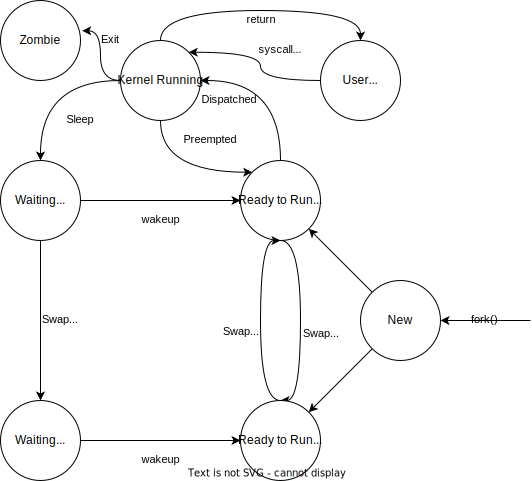
\includegraphics[width=\textwidth]{process_state}
	\caption{Process State Transition}\label{fig_process_state_diagram}
\end{figure}
\subsection{Process Control}
\subsubsection{Process Control Block}
\paragraph{Structure of Process Control Block}
\begin{enumerate}
	\item Process State: created, ready to run, run, asleep, zombie, preempted, orphan etc.
	\item PID: Unique ID of the process
	\item Program Counter: Address of the next instruction
	\item Registers: Stack Pointers, Index Registers etc.
	\item Memory Management Information: Paging, Segmentation etc.
	\item Scheduling Info: Priority of processes, the implemented algorithms etc. 
	\item Open file lists: The resources that are in use devices, files etc.
	\item Timing Info: Running time, Remaining CPU burst, CPU utilization.
\end{enumerate}
\paragraph{Some notable points}
\begin{itemize}
	\item implemented using \textbf{double linked list}
	\item each process has it's own PCB
	\item PCB of all processes stored in \textbf{main memory}
\end{itemize}

\subsection{Process Modes}
The primary goal of the dual mode operation is to provide protection and security to the user application programs and the
operating system from the unauthorized users. The mode bit is used to determine the particular mode in which an instruction
is executing.
\subsubsection{User Mode}
\begin{itemize}
	\item direct access to the hardware 
	\item full access to the machine instruction set
	\item I/O operations, context-switching, clearing the memory map
\end{itemize}

\subsubsection{Kernel Mode}
\begin{itemize}
	\item direct access to the hardware 
	\item full access to the machine instruction set
	\item I/O operations, context-switching, clearing the memory map
\end{itemize}

\subsubsection{Mode Switching} Steps involving switching between kernel mode and user mode\\
\begin{tabular}{|l|l|}
	\hline 
	Mode bit: 0 & Kernel mode \\ 
	\hline 
	Mode bit: 1 & User mode \\ 
	\hline 
\end{tabular} 

\subsection{Context}
\subsubsection{Context Switching}
\paragraph{What is Context Switching?}
A context switch is storing the state or context of a process so that it can be reloaded whenever required for execution from the same point it was switched as earlier. Context switches can occur only in kernel mode.
\subparagraph{The steps of context switching}
A typical thread context switch on a CPU happens like this:
\begin{enumerate}
	\item Save the context of the process that is currently running on the CPU.
	\item Update the process control block and other important fields.
	\item Move the process control block of the above process into the relevant queue such as the ready queue, I/O queue etc.
	\item Select a new process for execution.
	\item Update the process control block of the selected process. This includes updating the process state to running.
	\item Update the memory management data structures as required.
	\item Restore the context of the previous process by loading the old values of the process control block and registers loaded again on the processor
\end{enumerate}

\section{Process Scheduling}
\subsection{Process Schedulers}
\paragraph{Short Term Schedulers} Select a job from ready queue based on its policy and gives the control of the CPU to that process with the help of "Dispatcher". Also known as CPU scheduler.
\begin{itemize}
	\item $Ready \rightarrow Run$
\end{itemize}
\paragraph{Mid Term Schedulers} If a process requests an I/O in the middle of execution, then the process removed from the main memory is loaded into the waiting queue of secondary memory (\textbf{swap-out}). When the I/O operation is completed, then the job moved from waiting queue of secondary memory to ready queue (\textbf{swap-in}). Also known as swapper.
\begin{itemize}
	\item $Ready \leftrightarrow Suspend Ready$
	\item $Block \leftrightarrow Suspend Block$
\end{itemize}
\paragraph{Long Term Schedulers} Select a job from disk and decides whether it should load it into main memory or not. Choosing a good mix of CPU/IO bound processes is main task. Also known as job Scheduler.
\begin{itemize}
	\item $New \rightarrow Ready$
\end{itemize}
\paragraph{Dispatcher}
\begin{itemize}
	\item loading the job onto the CPU
	\item perform context-switching
\end{itemize}
\begin{figure}[H]
	\centering
	\includegraphics[width=\textwidth]{process_scheduler}
	\caption{Process Schedulers}\label{fig_process_scheduler_diagram}
\end{figure}

\subsection{CPU Scheduling Criteria} CPU Scheduling Criteria in OS
\paragraph{CPU Utilization $(\uparrow)$} This is the percentage of time that the processor is busy, CPU utilization may range from 0-100\%.
\paragraph{Throughput $(\uparrow)$} It means how many jobs are completed by the CPU.
\paragraph{Waiting Time $(\downarrow)$} Waiting time is the sum of the periods spent waiting by a process in the ready queue.
\paragraph{Response Time $(\downarrow)$} Response time is the time duration between the submission and the first response.
\paragraph{Turnaround Time} The time interval between the submission of the process and the time of the completion is the turnaround time. This is the turnaround time formula in OS [Turnaround time = Waiting time in the ready queue + executing time + waiting time in waiting-queue for I/O].
\paragraph{Arrival Time} time required from birth to the Ready state
\paragraph{Burst / Service Time} time required by the process to complete execution

\subsection{Process Scheduling Algorithms}
\paragraph{First Come First Serve (FCFS)}
\begin{itemize}
	\item This is a non-preemptive algorithm
	\item Use queue (FIFO) for implementation
    \item Free from Starvation
    \item Suffers from \textit{convoy effect}
\end{itemize}
\paragraph{Last Come First Serve (LCFS)}
\begin{itemize}
	\item This is a non-preemptive algorithm
	\item Use stack (LIFO) for implementation
\end{itemize}
\paragraph{Priority Based}
\begin{itemize}
    \item May be preemptive or non-preemptive
	\item Suitable for realtime systems where critical task to be finished first and deadline to be met
\end{itemize}
\paragraph{Shortest Job First (SJF)}
\begin{itemize}
	\item non-pre-emptive algorithm.
    \item Extension of priority scheduler, here highest priority is given to the process with smallest CPU burst time
    \item Large processes may starve
    \item CPU burst time is unknown at the time of arrival
    \item Minimizes average response time of processes
\end{itemize}
\paragraph{Shortest Remaining Task First (SRTF)}
\begin{itemize}
	\item preemptive algorithm
    \item shortest job at this instant is assigned to the CPU
    \item Large processes may starve
    \item Minimizes the average turnaround time of the processes
\end{itemize}
\paragraph{Round-Robin (RR)}
\begin{itemize}
	\item preemptive algorithm. 
	\item CPU has a fixed time quantum i.e. each Process is given a limited time to complete its task. If it gets completed within that fixed time or the time is over then the control of CPU is given to another process waiting in the queue. Creates a illusion that all processes is running at the same time.
	\item Used mainly in time-sharing systems.
	\item $ns + (n-1)q = t$ where n is number of jobs, s is process switching time, q is time quantum
\end{itemize}
\paragraph{Highest Response Ratio Scheduling (HRRS)}
\begin{itemize}
    \item non-preemptive algorithm.
    \item No starvation
    \item Processes are assigned to the CPU based on their highest response ratio
    \item $ResponseRatio=\frac{WT+BT}{BT}$, Favors jobs that are waiting longer    
    
\end{itemize}
\paragraph{Multilevel Queue}
\begin{itemize}
	\item Used both priority and round-robin scheduling
    \item Processes are put into multiple levels based on priority
    \item multiple processes in the highest-priority queue, are executed in round-robin order
    \item Common division Foreground Process (Realtime process, System process, interactive process), Background Process (batch process)
\end{itemize}
\paragraph{Multilevel Feedback Queue}
\begin{itemize}
	\item Processes moves between queue
    \item I/O-bound \& interactive processes which are typically characterized by short CPU bursts are put in the higher-priority queues if a process uses too much CPU time that demoted to low priority queue
\end{itemize}
\begin{table}[H]
	\begin{center}
		\begin{tabular}{|l|c|c|c|c|}
			\hline
			\rowcolor{gray!20}
			\thead{Scheduling Algorithm} & \thead{CPU Overhead} & \thead{Throughput} & \thead{TAT} & \thead{RT} \\
			\hline
			FIFO & LOW & LOW & HIGH & LOW \\
			\hline
			SJF & MEDIUM & HIGH & MEDIUM & MEDIUM \\
			\hline
			PRIORITY & MEDIUM & LOW & HIGH & HIGH \\
			\hline
			ROUND ROBIN & HIGH & MEDIUM & MEDIUM & HIGH \\
			\hline
		\end{tabular}
		\caption{Comparison between different scheduling}
		\label{tbl-scheduling-comparison}
	\end{center}
\end{table}

\section{Threading}
\subsection{Threading Concept}
\subsection{Thread Control Block}
\begin{itemize}
	\item \textbf{Thread ID} Unique ID for each thread.
	\item \textbf{Thread states} Current state of the thread
	\item \textbf{CPU information} Program Counters and Registers
	\item \textbf{Thread Priority} Priority of that thread
	\item A pointer which points to the process which triggered the creation of this thread.
	\item A pointer which points to the thread(s) created by this thread.
\end{itemize}
\subsection{Thread Types}
\subsubsection{Based on level}
\paragraph{Kernel level threads}
\begin{itemize}
	\item Kernel level threads are supported and managed directly by the operating system.
	\item The kernel knows about and manages all threads.
	\item One process control block (PCP) per process.
	\item One thread control block (TCB) per thread in the system.
	\item Provide system calls to create and manage threads from user space.
\end{itemize}

\subparagraph{Advantages}
\begin{itemize}
	\item The kernel has full knowledge of all threads.
	\item Scheduler may decide to give more CPU time to a process having a large number of threads.
	\item Good for applications that frequently block.
	\item The context size is more
	\item Hardware support is required
\end{itemize}

\subparagraph{Disadvantages}
\begin{itemize}
	\item Kernel manage and schedule all threads.
	\item Significant overhead and increase in kernel complexity.
	\item Kernel level threads are slow and inefficient compared to user level threads.
	\item Thread operations are hundreds of times slower compared to user-level threads.
\end{itemize}

\paragraph{User level threads}
\begin{itemize}
	\item User level threads are supported above the kernel in user space and are managed without kernel support.
	\item Threads managed entirely by the run-time system (user-level library).
	\item Ideally, thread operations should be as fast as a function call.
	\item The kernel knows nothing about user-level threads and manage them as if they where single-threaded processes.
	\item The context size is less
	\item No hardware support required
\end{itemize}

\subparagraph{Advantages}
\begin{itemize}
	\item Can be implemented on an OS that does not support kernel-level threads.
	\item Does not require modifications of the OS.
	\item Simple representation: PC, registers, stack and small thread control block all stored in the user-level process address space.
	\item Simple management: Creating, switching and synchronizing threads done in user-space without kernel intervention.
	\item Fast and efficient: switching threads not much more expensive than a function call.
\end{itemize}
\subparagraph{Disadvantages}
\begin{itemize}
	\item Not a perfect solution (a trade off).
	\item Lack of coordination between the user-level thread manager and the kernel.
	\item OS may make poor decisions like:
	\begin{itemize}
		\item scheduling a process with idle threads
		\item blocking a process due to a blocking thread even though the process has other threads that can run
		\item giving a process as a whole one time slice irrespective of whether the process has 1 or 1000 threads
		\item unschedule a process with a thread holding a lock.
	\end{itemize}
	\item May require communication between the kernel and the user-level thread manager (scheduler activation) to overcome the above problems.
\end{itemize}
\subsubsection{Based on Number}
\paragraph{Single-threading}
\paragraph{Multi-threading}
\subparagraph{Multi-Threading Model}
\begin{itemize}
	\item \textbf{One-to-One} Each user level thread is mapped to single kernel-level thread
	\item \textbf{Many-to-One} Many user level threads are mapped to single kernel-level thread.
	\item \textbf{Many-to-Many} Many user level threads are mapped to multiple kernel-level threads
\end{itemize}
\subparagraph{Disadvantages}
\begin{itemize}
	\item Blocking one user-level thread of a process blocks the entire process
	\item TCB is considered as overhead for the system
\end{itemize}
\section{Process Coordination}
\subsection{Process Communication}
\subsubsection{Types of Communication}
\begin{itemize}
	\item \textbf{Cooperative} Execution of one process affects or affected by other process
	\item \textbf{Independent} No communication between processes
\end{itemize}
\subsection{Problems arises for not having synchronization}
\subsubsection{Producer Consumer} %TBD
\subsubsection{Dining Philosopher Problem} %TBD
\subsection{Synchronization}
\subsubsection{Critical Section}
\begin{itemize}
	\item \textbf{Critical Section} The portion of program text where shared variables or shared resources will be placed.
	\item \textbf{Non-Critical Section} The portion of program text where the independent code of the processes will be placed.
	\item \textbf{Race condition} The final value of any variable depends on execution sequence of the processes in which access takes place.
	\item To avoid the Race condition, only one process is allowed to enter into critical section
\end{itemize}
\paragraph{Conditions for handling critical Section}
To prove that this solution is correct. All the following conditions to be satisfied. 
\begin{itemize}
	\item \textbf{Mutual Exclusion} Only one process is allowed to enter into critical section at any point of time
	\item \textbf{Progress} No process that are running in remainder section can choose who can run in the critical section. Selection cannot be postponed indefinitely
	\item \textbf{Bounded Waiting} No process should have to wait forever to enter into critical section, there should be a bound/limit or it will lead to starvation.
\end{itemize}
\subsubsection{Solutions for Critical Section Problem}
\paragraph{Peterson’s solution}
\begin{itemize}
    \item Classic Software based solution
    \item May or may not work on RISC systems    
    \item every processes given a number i
    \item the turn indicates which process's turn to enter into critical section
    \item flag indicates if a process want to enter in critical section
    \item always gives way to the other process
\end{itemize}
\begin{lstlisting}
    boolean flag[2];
    while (true) {
        flag[i] = true;
        turn = j;
        while (flag[j] && turn == j);
        /* critical section */
        flag[i] = false;
        /* remainder section */
    }
\end{lstlisting}

\begin{tabular}{|c|c|c|c|}
    \hline
    \thead{Algorithm Name} & \thead{Mutual Exclusion} & \thead{Progress} & \thead{Bounded Waiting} \\
    \hline
    Lock Variable & $\times$ & $\surd$ & $\times$ \\
    \hline
    Decker’s Algorithm & $\surd$ & $\times$ & $\surd$ \\
    \hline
    Peterson’s Algorithm & $\surd$ & $\surd$ & $\surd$ \\
    \hline
    TSL Instruction & $\surd$ & $\surd$ & $\times$ \\
    \hline
\end{tabular}
\subsubsection{Monitor}
\begin{itemize}
    \item Monitors is a programming language compiler support type of solution to achieve synchronization.
    \item Monitors is collection of variables and procedures combined together in a special kind of module or package.
    \item The process running outside the monitor cannot directly access the internal variables of the monitor but however they can call the procedures of the monitor.
    \item Monitors has an important property that only one process can be active inside the monitor at any point of time.
\end{itemize}
\subsubsection{Semaphore}
Semaphore is an integer variable which is used by the various processes in a mutual exclusive manner to achieve synchronization.
\begin{itemize}
    \item Down(); or wait (); or p ()
    \item up(); or signal (); or v (); or release ();
\end{itemize}
\paragraph{Binary Semaphore}
\paragraph{Counting Semaphore}

\subsection{Deadlock}
\subsubsection{Deadlock Characteristics}
\begin{itemize}
	\item \textbf{Mutual Exclusion} Each resource can be assigned to at most one process only.
	\item \textbf{Hold and Wait} Processes hold a resource and may seek an additional resource.
	\item \textbf{No Preemption} Processes that have been given a resource cannot be preempted to release their resources.
	\item \textbf{Circular Wait} Every process awaits release of at least one resource held by some other processes.
\end{itemize}

A deadlock can occur only when all four conditions are present simultaneously.
\subsubsection{Deadlock Prevention}
\paragraph{Methods for deadlock prevention}
Deadlock can be prevented by unsatisfying one of the deadlock characteristics
\begin{itemize}
    \item \textbf{Mutual Exclusion} cannot be unsatisfied because of the concept of sharable and non-sharable resources
    \item \textbf{Hold and Wait}
    \begin{itemize}
        \item A process should be assigned all the required resources before the start of its execution. This may lead to low device utilization
        \item The process should release all the existing resources before making a new request. This may eventually lead to starvation.
    \end{itemize}
    \item \textbf{No Preemption} A process will be put into waiting state if all the resources required by the process is not available. If a process is waiting then it's resources can be preempted, like "wound–wait"
    \item \textbf{Circular Wait} Similar resources will be marked uniquely, so it will behave like a single resource and when any two process requests it, then resources can be assigned based on process timestamp.
\end{itemize}

\subsubsection{Deadlock Detection}
\paragraph{Safe \& Unsafe States}
\begin{itemize}
    \item If a system is in safe state  $\Rightarrow$ no deadlocks.
    \item If a system is in unsafe state $\Rightarrow$ possibility of deadlock.
\end{itemize}
\paragraph{Resource Allocation Graph}
RAG is a directed graph whose nodes are either square(Resource) or circle(Process). An arc from circle to square means process is requesting for that resource. An arc from square to circle means process is holding that resource.


\subsubsection{Deadlock Avoidance}


\paragraph{Banker's Algorithm}
\begin{enumerate}
    \item Let Work and Finish be vectors of length 'm' and 'n' respectively.
    \begin{itemize}
        \item Initialize: Work = Available
        \item Finish[i] = false; for i=1, 2, 3, 4…,n
    \end{itemize}
    \item Find an i such that both
    \begin{itemize}
        \item Finish[i] = false
        \item Need i $<=$ Work
    \end{itemize}
    \item if no such i exists go to step (4)
    \item Work = Work + Allocation[i]
    \begin{enumerate}
        \item Finish[i] = true
        \item go to step (2)
    \end{enumerate}
    \item if Finish[i] = true for all i then the system is in a safe state
\end{enumerate}

\subparagraph{Limitations of Banker's Algorithm}
\begin{itemize}
    \item Banker's algorithm can't eliminate an existing deadlock.
    \item Resource requirements must be are known beforehand.
    \item Number of live processes and resources are limited.
    \item Process synchronization is not possible because it doesn't guarantee any particular sequence.
\end{itemize}
\chapter{Memory Management}
\section{Basics}
\subsection{Partition}
\subsection{Fragmentation}
\subsection{Swapping}
\subsection{Thrashing}
\subsection{Demand Paging}
\section{Virtual Memory}
\subsection{Paging}
\subsection{Page Tables}
\subsection{Page Faults}
\subsection{Page Replacement}
\paragraph{Optimal Page replacement}
\paragraph{LRU}
\paragraph{LFU}
\paragraph{FIFO}
\paragraph{Second Chance}
\paragraph{Clock}

\chapter{Storage Management}
\section{Disk Management}
\subsection{Disk Components}
\begin{itemize}
\item \textbf{Platter} The surface of a magnetic disk is known as platter.
\item \textbf{Track} The surface of a platter is  logically divided into circular shapes known as tracks.
\item \textbf{Sector} Tracks are divided into smaller sections known as sectors.
\item \textbf{Cylinder} A set of tracks that are at one arm position are called cylinders.
\end{itemize}
\paragraph{Relations Between Above}
$$ SingleTrackDataCapacity = SectorsPerTrack * BytesPerSector $$
$$ TransferSpeed = \frac{RPM}{60} * SingleTrackDataCapacity $$
\paragraph{Disk Timings}
\begin{itemize}
	\item \textbf{Seek Time}
	\item \textbf{Access Time}
	\item \textbf{Latency}
\end{itemize}
\subsection{Disk Scheduling Algorithms}
\paragraph{FCFS (First Come First Serve)}
\paragraph{SSTF (Shortest Seek Time First)}
\paragraph{SCAN \& CSCAN}
\paragraph{LOOK \& CLOOK}
\begin{table}[H]
	\begin{center}
		\begin{tabular}{|l|c|c|}
			\hline
			\rowcolor{gray!20}
			\thead{Algorithm} & \thead{Advantages} & \thead{Disadvantages} \\
			\hline
			FIFO &  & LOW \\
			\hline
			SSTF & MEDIUM & HIGH\\
			\hline
			SCAN/LOOK & MEDIUM & LOW \\
			\hline
			C-SCAN/C-LOOK & HIGH & MEDIUM\\
			\hline
		\end{tabular}
		\caption{Comparison between different disk scheduling}
		\label{tbl-disk-sch-comparison}
	\end{center}
\end{table}

\section{File Management}
\subsection{File Systems}
\paragraph{Floppy Disk FS}
\paragraph{FAT}
\paragraph{NTFS}
\paragraph{EXT}

\chapter{Protection \& Security}
\chapter{Special Systems}
\section{Windows XP}
\section{Linux OS}
\section{Mac OS}
\section{Android OS}
\section{Distributed System}
\section{Real-time System}

% System calls, processes, threads, inter‐process communication, concurrency and synchronization.
% Deadlock. CPU and I/O scheduling. Memory management and virtual memory. File systems.

%\paragraph{RAID} Redundant Array of Independent Disk is a technique that focuses on fault tolerance using replication of same data. Raid use mirroring and also error correction this is done mainly using checksum.
%\begin{figure}[H]
%	\centering
%	\includegraphics[width=\textwidth]{storage_raid_levels}
%	\caption{Traditional RAID Levels}\label{fig_raid_table}
%\end{figure}

%Look ahead buffer
%Look aside buffer

%Reread Questions:
%Disks: GATE1997-74
%Disks: GATE2004-49
%User level-threads, kernel supported threads
\part{Computer Networking}
\chapter{Introduction to computer Networks}
\section{Problems associated with Computer Networks}
\subsection{Communication}
\paragraph{Protocols}
Protocol is set of rules that govern data communications.\\
\indent \textbf{Syntax:} The term refers to the structure or format of the data, meaning the order in which they are presented.\\
\indent \textbf{Semantics:} The term refers to the meaning of each section of bits. How are a particular pattern to be interpreted, and what action is to be taken based on that interpretation?\\
\indent \textbf{Timing:} The term refers to two characteristics: a) When data should be sent b) How fast they can be sent.
\subparagraph{HTTP} (\textbf{Hyper Text Transfer Protocol}) Used for browser requesting resources from a server. Available versions are: 1.0 (\textit{RFC 1945}), 2.0 (\textit{RFC 7540}). Methods available are: GET, HEAD, POST, PUT, DELETE, CONNECT, OPTIONS, TRACE, PATCH etc. Port used: 80 and 443 (secure). This is a TCP protocol.
\subparagraph{SMTP} (\textbf{Simple Mail Transfer Protocol}) Used for Delivering mails to servers. Available in \textit{(RFC 821)}. Available methods are: HELO, MAIL, RCPT, SEND, DATA, VRFY, AUTH, RSET, QUIT etc. Port used: 25. This is a TCP protocol.
\subparagraph{FTP} (\textbf{File Transfer Protocol}) Used for downloading or uploading file from or to server. Available in \textit{(RFC 959)}. Available methods are the common file handling commands of UNIX system. Port used: 20/21. This is a TCP protocol.
\subparagraph{POP} (\textbf{Post Office Protocol}) Client connect, retrieve, store them and finally delete them from server. Available in POP \textit{(RFC 918)}, POP3 \textit{(RFC 1081)}. Available methods are: USER, PASS, QUIT, STAT, RETR, DELE, RSET etc. Port used: 110 and 995 (secure).
\subparagraph{IMAP} (\textbf{Internet Message Access Protocol}) Used for complete management of mailbox. User can download a message using different clients and keep a copy on the server until explicitly deleted. Available in \textit{(RFC 3501)}. Available methods are: APPEND, CHECK, SEARCH, SELECT, STORE etc. Port used: 143 and 993 (secure).
\subparagraph{TELNET} (\textbf{TELetype NETwork}) Provides a bidirectional interactive text-oriented communication facility. Available in \textit{(RFC 15)}. Available methods are: CLOSE, DISPLAY, OPEN, SET, SEND, STATUS, UNSET, QUIT etc. Port used: 23. This is a TCP protocol.
\subsection{Identification}
To send packets from source to destination we need to identify systems. Two types of addressing are used for this: a) Logical address (IP) and b) Physical addressing (MAC)
\paragraph{IP Address}
\subparagraph{Characteristics of IP address}
\subparagraph{Classification of IP address\\}

\begin{tabular}{|p{2em}|p{2em}|p{3em}|p{8em}|p{10em}|}
	\hline IP Class & NID-HID & Starting bits & Range & Area of usage \\
	\hline A & 8-24 & 0 & 1.0.0.1 to 126.255.255.255 & Defense, Govt organizations etc.\\
	\hline B & 16-16 & 10 & 128.0.0.1 to 191.255.255.255 & MNC, Banks, Big organizations etc.\\
	\hline C & 24-8 & 110 & 192.0.0.1 to 223.255.255.255 &  etc.\\
	\hline D & nil & 1110 & 224.0.0.1 to 239.255.255.255 & Used for multi-casting purposes\\
	\hline E & nil & 11110 & 240.0.0.1 to 255.255.255.255 & Reserved for future uses\\
	\hline
\end{tabular}

\subparagraph{Some special IP addresses} 
\textbf{127.*.*.*} is reserved for  loop-back.
\paragraph{MAC Address}
\subsection{Connection}
\paragraph{Types of Connections}
\subparagraph{Uni-casting}
When source is sending data to only one device.
\subparagraph{Multi-casting}
When source is sending data to multiple devices.
\subparagraph{Broadcasting}:

\textbf{Limited Broadcasting:} A packet is sent to a specific network or series of networks.

\textbf{Directed Broadcasting:} A packet is sent to specific destination address.

\textbf{Flooded Broadcasting:} A packet is sent to every network.
\paragraph{Netting}
\subparagraph{Subnetting}
\subparagraph{Supernetting}
\paragraph{Hardware Devices}
\subparagraph{Repeater (PL)} It receives signals and either amplifies or regenerate it.
\subparagraph{Hub (PL)} Passive Broadcasting device no s/w needed.
\subparagraph{Bridge (PL, DL)} Connects multiple LAN segments (similar) or subnets 
\subparagraph{Switch}
\subparagraph{Router}
\subparagraph{Gateway}
\chapter{Layers of computer Networks}
Here is a Cheat-sheet for Layers of OSI model:\\
\begin{tabular}{|p{5em}|p{10em}|p{3em}|p{8em}|}
	\hline Layer Name & Objectives & PDUs & Protocols\\
	\hline Application Layer & Bla Bla & Bla & DNS, HTTP, FTP, DHCP, IMAP, LDAP, POP, RSTP, RIP, SMTP, SNMP, SSH, TelNet, SIP, TLS/SSL,\\
	\hline Presentation Layer & Bla Bla & Bla & DNS, HTTP, FTP, DHCP, IMAP, LDAP, POP, RSTP, RIP, SMTP, SNMP, SSH, TelNet, SIP, TLS/SSL,\\
	\hline Session Layer & Bla Bla & Bla & DNS, HTTP, FTP, DHCP, IMAP, LDAP, POP, RSTP, RIP, SMTP, SNMP, SSH, TelNet, SIP, TLS/SSL,\\
	\hline Transportation Layer & Bla Bla & BLA & TCP, UDP, DCCP, SCTP, RSVP\\
	\hline Network Layer & Bla Bla & BLA & IPv4, IPv6, IGMP, IPsec, ICMP\\
	\hline Data Link Layer & Bla Bla & BLA & ARP, NDP, L2TP. PPP, DSL, ISDN, FDDI \\
	\hline Physical Layer & Bla Bla & BLA & ARP, NDP, L2TP. PPP, DSL, ISDN, FDDI \\
	\hline
\end{tabular}
\section{Application Layer}
\section{Presentation Layer}
\section{Session Layer}
\section{Transport Layer}
\section{Network Layer}
\section{Data Link Layer}
\subsection{Error Control}
\textbf{Error:} During transmission when bits or signal gets changed, called error.\\
\textbf{Single-bit Error:} When only one bit gets changed.\\
\textbf{Burst Error:} When 2 or more bits get changed.
\paragraph{Parity Checking} Adding redundant bits to the end of actual data, called parity bits. During sending of data the parity bits are calculated using XOR operation for even parity and XNOR for odd parity. In the receiving end they parity is calculated again if 0 then there is no error so remove the parity bits and accept data else reject and request again.
\paragraph{Hamming Code} In this mechanism to get the final data we need to ind the parity bit of those which have 1's in $n^{th}$ position and add them to the $2^n$ position. The number of redundant bits needed are: $2^{n+1} > len(Code)$. On the receiving end recalculate the hamming code, if result is all 0's then accept the data, else alter the bit position of the result to get the error free data as it is a error detection and correction code. This can detect more than 1 bit error but cannot correct them.
\paragraph{Cyclic Redundancy Check} To get the redundant bits, data is divided with a prime divisor. The remainder is added to the data. On the receiving end, the modified data is also divided by the same divisor. If remainder is 0 then accept the data, else reject the data.
\paragraph{Checksum} Data are divided into same size segments with the help of padding, then summed together. The result is then inverted and send with the actual data. On the receiving end, the data received is again divided and summed up if resulted in 0 then data is correct else reject the data.
\subsection{Data Link Control}
\paragraph{Framing}  Helps to identify messages from different sources and destinations. It has three main parts: HEADER, containing control information, source and destination addresses, type of PDU, Control fields; DATA, contains content of the packets; TRAILER, contains error control bits, stop bits.
\subparagraph{Character Oriented Framing} Data are sent in byte format.\\
\indent \indent \textbf{Default structure:} Flag + Header + ... Data ... + Trailer + Flag\\
\indent \indent \textbf{Byte Stuffed:} ESC bytes are added before every FLAG and ESC in the data. e.g. \textit{Flag + Header + ... ESC FLAG ... Data ... ESC ESC ... + Trailer + Flag}
\subparagraph{Bit Oriented Framing}
\indent \indent \textbf{Default structure:} Flag + Header + ... Data ... + Trailer + Flag\\
\indent \indent \textbf{Bit Stuffed:} ESC bytes are added before every FLAG and ESC in the data. e.g. \textit{Flag + Header + ... ESC FLAG ... Data ... ESC ESC ... + Trailer + Flag}
\subsection{Flow Control}
\paragraph{Noiseless Channel}
\paragraph{Noisy Channel}
\subparagraph{Stop and wait protocol}
\subparagraph{Go-back-N protocol}
\subparagraph{Selective repeat protocol}
$TransmissionDelay=\frac{FrameSize}{Bandwidth}$ $OptimalSenderWindowSize=1+2a=1+2*\frac{PropagationDelay}{TransmissionDelay}$ $min.SequenceNumberBits=\lceil log_2(OptimalSenderWindowSize+OptimalReceiverWindowSize)\rceil$
\subsection{Access Control}
\paragraph{Random Access Control}
\paragraph{Controlled Access Control}
\paragraph{Channelization Control}
\section{Physical Layer}
\subsection{Data and Signals}
\paragraph{Signals}
\subparagraph{Different Types of Signals}:\\
\indent \textbf{Analog Signals} It includes an infinite number of values along its path.\\
\indent \textbf{Digital Signals} It includes limited number of defined values along its path.\\
\indent \textbf{Periodic Signals} It repeats patterns in a common time frame.\\
\indent \textbf{Non-periodic Signals} It doesn't repeat any pattern.\\
\indent \textbf{Analog Data} It refers to information that is continuous.\\
\indent \textbf{Digital Data} It refers to information that is discrete in nature.\\
(*) Periodic analog signals and non-periodic digital signals are commonly used.
\subparagraph{Different Properties of Analog Signals}:\\
\indent \textbf{Period and Frequency:} The time needed to complete 1 cycle is called period (T). Frequency (f) means to the number of periods in 1s. i.e. $ f=\frac{1}{T} $.\\
\indent \textbf{Phase:} It denotes position of the signal relative to time 0. i.e. if $\frac{1}{C} $ is offset related to $time_0$ $d=360*\frac{1}{C}$.\\
\indent \textbf{Wavelength:} The distance a signal travels before completing a cycle is called wave lengths. $wavelength = PropagationSpeed * period = \frac{PropagationSpeed}{frequency}$.\\
\indent \textbf{Composite Signal:} Combination of different analog sine waves is called composite signal.\\
\indent \textbf{Bandwidth:} The difference between highest and lowest frequency of a composite signal.\\
\subparagraph{Different Properties of Digital Signals}:\\
\indent \textbf{Bit rate:} The number of bits send per second is called bit rate.\\
\indent \textbf{Bit Length:} Distance 1 bit occupies in the medium. i.e. $BitLength = PropagationSpeed * BitDuration$.
\indent \textbf{Throughput:} How fast we can send data though network. If a channel carries F frames per second and B bits per frame then throughput T = F * B.\\
\indent \textbf{Latency:} Total time taken to send first bit to entire message. Calculation: $Latency = PropagationTime + TransmissionTime + QueuingTime + ProcessingDelay;$
$PropagationTime = \frac{Distance}{PropagationSpeed};$
$TransmissionTime = \frac{MessageSize}{Bandwidth}$. \\
\subparagraph{Anomalies during transmission}:\\
\indent \textbf{Attenuation:} During traveling through medium signal loses its energy is called attenuation. Calculation: $dB=10log_{10}\frac{P_e}{P_s}$\\
\indent \textbf{Distortion:} When signals changes its form or shape.\\
\indent \textbf{Noise:} When impurities from outside of medium corrupts the signal is called noise. $SNR_{dB}=10log_{10}SNR=10log_{10} \frac{AvgSignalPower}{AvgNoisePower}$\\
\paragraph{Transmission of Signals}
\subparagraph{Conversions}
\subparagraph{Transmission Modes}:\\
\indent \textbf{Parallel Transmission:} n-wires send n-bits of data at same time mostly binary data 0 and 1. Normally used when distance is too short as it costs more.\\
\indent \textbf{Serial Transmission:} Data are transmitted serially\\
\indent \indent \textbf{Asynchronous:} Units of bits are send begin with start bit(0) and end with stop bits(1). Data bits are asynchronous at byte level.\\
\indent \indent \textbf{Synchronous:} Data bits are combined and send as frames one after another and receiver has the job to separate those bits into groups.\\
\subparagraph{Multiplexing} Bandwidth is shared if a medium got higher bandwidth than the needs of devices this technique is called multiplexing.\\
\indent \textbf{Frequency Division Multiplexing:} An analog method is used to combine signals. Different frequencies are separated by the guard-bands to prevent overlapping.\\
\indent \textbf{Time Division Multiplexing:} Data from different slow-rate devices are given a fixed time slots in round robin manner to achieve high-rate.\\
\indent \textbf{Wave Division Multiplexing:} Designed for Optic Fiber, uses the technique of refraction.\\
\subsection{Transmission Medium}
\paragraph{Guided Media}
\subparagraph{Twisted Pair Cable} A twisted pair of conductors each with own plastic insulation.
\subparagraph{Co-axial Cable}  
\subparagraph{Optic Fiber Cable}
\paragraph{Unguided Media}
\subparagraph{Radio wave}
\subparagraph{Micro wave}
\subparagraph{Infrared wave}
\subsection{Switching}
\paragraph{Circuit Switching} Switches connected through actual links and circuits. Reserve all the resources during transmission. Implemented in physical layer.
\paragraph{Packet Switching} Data are arranged into packets and then send over network. Resources are allocated as they needed. Each switch has routing table.
\subparagraph{Datagram Networks} Packets are sent independent of each other. Normally switching done in network layer and called connection-less. Each have a routing table contains destination address and output port.
\subparagraph{Virtual Circuit Networks} During setup phase the path is selected, all packets follow same path to reach destination. Normally implemented in data-link layer and called connection-oriented. Routing table consists of incoming/outgoing ports/VCI.
\chapter{Network Security}
\chapter{Mobile Technologies}
\chapter{Cloud Computing}
\chapter{Not Sorted}
\section{IP}
To check an IP belongs to same network, do AND(.) operation between subnet mask and IP.\\
\textbf{CIDR representation} is IP/C. To find the range do $N = 32-C$. Truncate last N bits to 0s for lowest IP and to 1s for highest IP and total IPs will be $2^N$.\\
\textbf{CIDR aggregation:} 1) All IPs must be contiguous. 2) Calculate total IP addresses. 3) Aggregated CIDR will be IP/X where, $X = 32-log_2T$.\\
\textbf{IP Fragmentation:} 1) Calculating $ActualTransmissionSize = MaximumTransmissionUnit - IPHeaderSize$ 2) Calculating $NumberOfSegments = \frac{TotalPacketSize}{ActualTransmissionSize} $ 3) Calculating $Offsets_i = \frac{ActualTransmissionSize}{8}*i  ;$ Initial offset is always 0.
\textbf{Hamming Code:} 1) Calculating $Min.HammingDistance=min_1(XORofEachCodewords)$ 2) Calculating $Max.ErrorBits=\frac{Min.HammingDistance-1}{2}$
\textbf{CSMA/CD:} 1) Calculating $RoundedTurnaroundTime = 2* PropagationDelay$ 2) Calculating $min.FrameSize = RoundedTurnaroundTime*Bandwidth$\\
\textbf{DHCP (Dynamic Host Configuration Protocol):} Assign IP addresses automatically, Centralized, Works on port UDP 67 and 68, Application Layer protocol, Supports both IPv4 and IPv6, Sometimes behaves as router.\\
\textbf{SLIP(SeriaL IP):} IP Encapsulation over Serial Ports, Replaced later by PPP, preferred for micricontrollers due to small overhead but not good for PCs.\\
\textbf{SNMP (Simple Network Management Protocol):} Management and Monitoring of networks, Application layer protocol, Uses ports UDP 161 and 162.\\
\textbf{IGMP(Internet Group Multi-casting Protocol):} Uses IPv4, manage by IP Encapsulation.\\
\textbf{IGMP(Internet Control Message Protocol):} Uses IPv6, manage by Multi-cast Listener Discovery\\
\textbf{ARP(Address Resolution Protocol):} Find out MAC address from IPv4, works on Layer 2 to 3, replaced by NDP in IPv6\\
\textbf{RARP(Reverse Address Resolution Protocol):} Find out IP address from MAC, works on Layer 3 to 2, replaced by BOOTP7 then DHCP in IPv6\\
\textbf{TCP congestion control:}
\textbf{Slow start} size of the congestion window increased exponentially until threshold.
\textbf{Congestion avoidance} size of the congestion window increased additively until threshold.
\textbf{Congestion detection} size of the threshold dropped to half (multiplicative decrease).
\part{Database Design}

\chapter{Introduction}
\section{Background}
\paragraph{Data} are the known facts that can be recorded and that have implicit meaning
\paragraph{Information}
\paragraph{Database}

\section{Database Architecture}
\subsection{Terminologies}
\begin{itemize}
	\item \textbf{X}
\end{itemize}
\section{Database}

\chapter{Relation Model}
\section{Relation}
\subsection{Terminologies}
\begin{itemize}
	\item \textbf{Relation} A relation is a table with columns and rows. (File)
	\item \textbf{Tuple} A tuple is a row of a relation. (Record)
	\item \textbf{Attribute} An attribute is a named column of a relation. (Field)
	\item \textbf{Arity/Degree} Number of attributes of database table.
	\item \textbf{Cardinality} Number of tuple of database table.
	\item \textbf{Domain} A domain is the set of allowable values for one or more attributes.
	\item \textbf{Base Relation} A named relation corresponding to an entity in the conceptual schema, whose tuples are physically stored in the database.
	\item \textbf{View} The dynamic result that is provides a virtual relation that may or may not exists and produced upon users' request
	\item \textbf{Relational database} A collection of normalized relations with distinct relation names
	\item \textbf{Relational Schema} A named relation defined by a set of attribute and domain name pairs.
	\item \textbf{Relational Database Schema} A set of relation schemas, each with a distinct name.
	\item \textbf{Key} Attribute or set of attribute is called key.
	\item \textbf{Super key} An attribute, or set of attributes, that uniquely identifies a tuple within a relation
	\item \textbf{Candidate Key} A superkey such that no proper subset is a superkey within the relation. It has two properties \textit{Uniqueness}, \textit{Irreducibility}, For any RDBMS table there must be atleast one candidate key, whose field value can not be null..
	\item \textbf{Overlapped Candidate Key}: Two or more candidate key with some common attribute.
	\item \textbf{Compound Candidate Key}: A candidate key with atleast two attributes.
	\item \textbf{Prime Attribute} the attributes that are part of a candidate key, a relation can have multiple candidate key but all may not contain same prime attribute.
	\item \textbf{Non-prime attribute} the attribute that does not belongs to any of the candidate keys of the relation.
	\item \textbf{Primary Key} A primary key is the candidate key chosen for use in identification of tuples
	\item \textbf{Null} Represents a value for an attribute that is currently unknown or is not applicable for this tuple.
	\item \textbf{Entity Integrity} In a base relation, no attribute of a primary key can be null.
	\item \textbf{Referential integrity} If a foreign key exists in a relation, either the foreign key value must match a candidate key value of some tuple in its home relation or the foreign key value must be wholly null.
	\item \textbf{Constrains} Additional rules specified by the users or database administrators of a database that define or constrain some aspect of the enterprise.
\end{itemize}

\section{E-R Model}
\section{}
\section{Query Language}

\chapter{Database Analysis \& Design}
\section{Modeling}
\section{Normalization}
\section{Query Processing}
\section{Query Optimization}

\chapter{Storage and Indexing}
\section{Physical Storage Systems}
\section{Data Structure}
\subsection{File Organization}
\section{Indexing}

\chapter{Transaction Management}
\section{Transactions}
\section{Concurrency}
\section{Recovery}

\chapter{Special Databases}
\section{Distributed Database}
\section{Semi-structured Database}
\section{Blockchain Database}
\part{Emerging Technologies}
\chapter{Artificial Intelligence}
\chapter{Web Technologies}
\chapter{Data Mining and Warehousing}
\chapter{Blockchain}
\chapter{Cloud Computing}
\chapter{Internet of Things}
\section{Device}
\subsection{Bluetooth}
\subsubsection{Introduction to Bluetooth}
\paragraph{What is Bluetooth?}
\begin{itemize}
    \item Wireless technology standard for short-range communication
    \item Operates in the 2.4 GHz ISM band
    \item Uses radio waves for data transmission
\end{itemize}

\paragraph{Purpose and Uses of Bluetooth}
\begin{itemize}
    \item \textbf{Wireless Data Transfer:}
    \begin{itemize}
        \item Share files, photos, contacts between devices
        \item Bluetooth Object Push Profile (OPP) for file sharing
    \end{itemize}
    \item \textbf{Audio Streaming:}
    \begin{itemize}
        \item Stream audio to headphones, speakers, car systems
        \item A2DP (Advanced Audio Distribution Profile) for high-quality audio
    \end{itemize}
    \item \textbf{Hands-Free Communication:} 
    \begin{itemize}
        \item Bluetooth headsets, car kits, earphones for hands-free calls
        \item HFP (Hands-Free Profile) for call control
    \end{itemize}
    \item \textbf{Peripheral Device Connection:} 
    \begin{itemize}
        \item Connect keyboards, mice, printers, game controllers wirelessly
    \end{itemize}
    \item \textbf{IoT Devices:}
    \begin{itemize}
        \item Used in smart home devices (e.g., lights, locks, thermostats)
        \item Bluetooth Low Energy (BLE) for low-power IoT communication
    \end{itemize}
    \item \textbf{Health Monitoring:}
    \begin{itemize}
        \item Sync fitness trackers, heart rate monitors, smartwatches
    \end{itemize}
    \item \textbf{Location-Based Services:}
    \begin{itemize}
        \item BLE beacons for indoor navigation, proximity marketing
    \end{itemize}
    \item \textbf{Automotive Applications:}
    \begin{itemize}
        \item Hands-free calls, music streaming in cars
    \end{itemize}
    \item \textbf{Gaming:}
    \begin{itemize}
        \item Wireless controllers for gaming consoles, smartphones
    \end{itemize}
\end{itemize}
\subsubsection{How Bluetooth Works?}
\paragraph{Key Concepts}
\begin{itemize}
    \item \textbf{Pairing Process:} \\
    - Devices need to pair by discovering and authenticating each other (PIN or passkey)
    \item \textbf{Frequency Hopping:} \\
    - Bluetooth uses \textbf{79 channels} in the 2.4 GHz band
    - Avoids interference by hopping between channels at 1600 times per second
    \item \textbf{Profiles and Protocols:} \\
    - Defines data types and communication methods (e.g., A2DP for audio, SPP for data transfer)
    - \textbf{L2CAP} protocol handles basic data transmission
    \item \textbf{Security:} \\
    - Uses \textbf{encryption} and \textbf{authentication} to secure data
    - Security modes: Just Works, Numeric Comparison, Passkey Entry
\end{itemize}
\subsubsection{Bluetooth Versions and Evolution}
\subsubsection{Bluetooth in Modern Devices}
\subsubsection{Bluetooth Security}
\subsubsection{Advantages of Bluetooth}
\subsubsection{Challenges and Limitations}
\subsubsection{Future of Bluetooth}
\chapter{UI/UX Design}
\appendix
\chapter{Abbreviations}
\section{Random}
\textbf{SPOOL} Simultaneous Peripheral Operations On-Line
\textbf{PCS} Process Contention Scope
\textbf{SCS} System Contention Scope
\textbf{AFH} Adaptive frequency-hopping spread spectrum
\textbf{RSSI} Received signal strength indicator

\backmatter
\printbibliography
\end{document}